\documentclass[aspectratio=169]{beamer}
%\usecolortheme{beaver}
\usepackage[english,ukrainian]{babel}
\usepackage{hyperref}
\hypersetup{colorlinks,urlcolor=blue}
\makeatletter
\DeclareUrlCommand\ULurl@@{%
  \def\UrlFont{\ttfamily\color{blue}}%
  \def\UrlLeft{\uline\bgroup}%
  \def\UrlRight{\egroup}}
\def\ULurl@#1{\hyper@linkurl{\ULurl@@{#1}}{#1}}
\DeclareRobustCommand*\ULurl{\hyper@normalise\ULurl@}
\makeatother
\usepackage[table]{colortbl}
\usecolortheme{whale}
\usepackage{etoolbox,refcount}
\usepackage{multicol}

\newcounter{countitems}
\newcounter{nextitemizecount}
\newcommand{\setupcountitems}{%
  \stepcounter{nextitemizecount}%
  \setcounter{countitems}{0}%
  \preto\item{\stepcounter{countitems}}%
}
\makeatletter
\newcommand{\computecountitems}{%
  \edef\@currentlabel{\number\c@countitems}%
  \label{countitems@\number\numexpr\value{nextitemizecount}-1\relax}%
}
\newcommand{\nextitemizecount}{%
  \getrefnumber{countitems@\number\c@nextitemizecount}%
}
\newcommand{\previtemizecount}{%
  \getrefnumber{countitems@\number\numexpr\value{nextitemizecount}-1\relax}%
}
\makeatother    
\newenvironment{AutoMultiColItemize}{%
\ifnumcomp{\nextitemizecount}{>}{3}{\begin{multicols}{2}}{}%
\setupcountitems\begin{itemize}}%
{\end{itemize}%
\unskip\computecountitems\ifnumcomp{\previtemizecount}{>}{3}{\end{multicols}}{}}
\usepackage[utf8]{inputenc}

\title{Формування дивідендної політики корпорації (на прикладі компаній, що входять до індексу Standard \& Poor's 100)}
\author{Студент 2 курсу магістратури\\спеціальності 072 «Фінанси, банківська справа та страхування»\\ОП «Корпоративні фінанси» Тараба В. С.\\ Науковий керівник: д. е. н., доцент Любкіна О. В.}
\institute{Київський національний університет імені Тараса Шевченка\\Економічний факультет\\Кафедра фінансів}

\begin{document}
	
\begin{frame}
\titlepage
\end{frame}

\begin{frame}
\frametitle{План презентації}
\setbeamertemplate{section in toc}[circle]
%\setbeamercolor{section in toc}{fg=UniBlue}
%\setbeamercolor*{section in toc}{fg=UniBlue}
\tableofcontents
\end{frame}

\section{Опис дослідження}

\begin{frame}
\frametitle{Опис дослідження}
\begin{itemize}
\item \alert {Метою дослідження} є визначення видів дивідендної політики на основі даних для компаній, що входять до індексу S&P 100.
\tinyskip
\item \alert {Об’єктом дослідження} є компанії, що входять до індексу S&P 100.
\tinyskip
\item \alert {Предметом дослідження} є види дивідендної політики та їх практична реалізація.
\tinyskip
\item \alert {Завданнями дослідження} є:
\begin{itemize}
    \item[\textcolor{orange}{\textbullet}] розглянути теоретичні засади формування дивідендної політики (основні чинники, що впливають на формування дивідендної політики компаній, види дивідендної політики та їх особливості); 
    \item[\textcolor{orange}{\textbullet}] розглянути можливості для автоматизації процесу збору та обробки та даних та обрати оптимальний варіант; 
    \item[\textcolor{orange}{\textbullet}] сформувати критерії для визначення видів дивідендної політики на основі даних;
    \item[\textcolor{orange}{\textbullet}] виконати збір даних за останні 10 років (2014-2023 рр), які необхідні для визначення виду дивідендної політики;
    \item[\textcolor{orange}{\textbullet}] визначити види дивідендної політики компаній, що входять до індексу S\&P 100
\end{itemize}
\end{itemize}
\end{frame}


\section{Ключові фінансові індикатори видів дивідендної політики}
\begin{frame}
\begin{itemize}
\item При визначенні видів дивідендної політики компаній будемо використовувати три показники: \alert {DPS} (дивіденди на одну звичайну акцію), \alert {EPS} (чистий прибуток на одну звичайну акцію), та розрахований на основі цих показників \alert {DPS} коефіцієнт виплати дивідендів (DPR), Також за потреби поділ акцій (спліт) та зворотній спліт будуть враховуватися при розрахунку \alert {коефіцієнта для корегування історичних показників}:
\[c=\prod_{i=1}^{n}k_{i}=e^{\ln\prod_{i=1}^{n}k_{i}}=e^{\sum_{i=1}^{n}\ln k_{i}}, k_{i}>0\]
де $k_{i}$ - коефіцієнт при спліті,який може набувати значень $0<k<1$  для звичайного спліту та $k>1$ для зворотнього спліту.
\smallskip
\item На основі аналізу літератури викоремлено 7 основних \alert {видів
дивідендної політики}: стабільного відсотка дивідендних виплат, фіксованого дивіденду, фіксованого дивіденду з преміальними виплатами, прогресивна, регресивна, нульового дивіденду, 100\% дивіденду.
\end{itemize}
\frametitle{Ключові фінансові індикатори видів дивідендної політики}
\end{frame}

\section{Збір та підготовка даних (формування бази даних)}
\begin{frame}
\begin{itemize}
\item Для збору, обробки даних,та розрахунків використовувалися \textcolor{blue} {python, SQL (SQL Server Management Studio) та Microsoft Power BI Desktop}.
\bigskip
\item \alert {Процес збору і обробки даних} складається з 4 основних етапів.
\begin{itemize}
    \item[\textcolor{orange}{\textbullet}] отримання списку тікерів, що входять до S&P 100 та загальної інформації для кожного тікеру (назва компанії, галузь тощо);
    \item[\textcolor{orange}{\textbullet}] збір по показниках DPS (дивіденди на одну звичайну акцію), EPS (чистий прибуток на одну звичайну акцію);
    \item[\textcolor{orange}{\textbullet}] приведення до єдиного формату та звірка показників, отриманих з різних джерел, для гарантування якості даних;
    \item[\textcolor{orange}{\textbullet}] розрахунок DPR (коефіцієнт виплати дивідендів) та побудова Power BI звіту на основі зібраних даних для визначення видів дивідендної політики та аналізу отриманих результатів.
\end{itemize}
\bigskip
\item \alert {Основними джерелами даних} є сайти finance.yahoo.com, stockanalysis.com, macrotrends.com, nasdaq.com; додаткові джерела даних:* sec.gov, investing.com, morningstar.com та сайти компаній.
\end{itemize}
\bigskip
\scriptsize \textcolor{gray}{* використовувалися лише за потреба в окремих випадках} 
\frametitle{Збір та підготовка даних (формування бази даних)}

\end{frame}

\begin{frame}
\frametitle{Формування бази даних (спрощена версія)}
\begin{center}
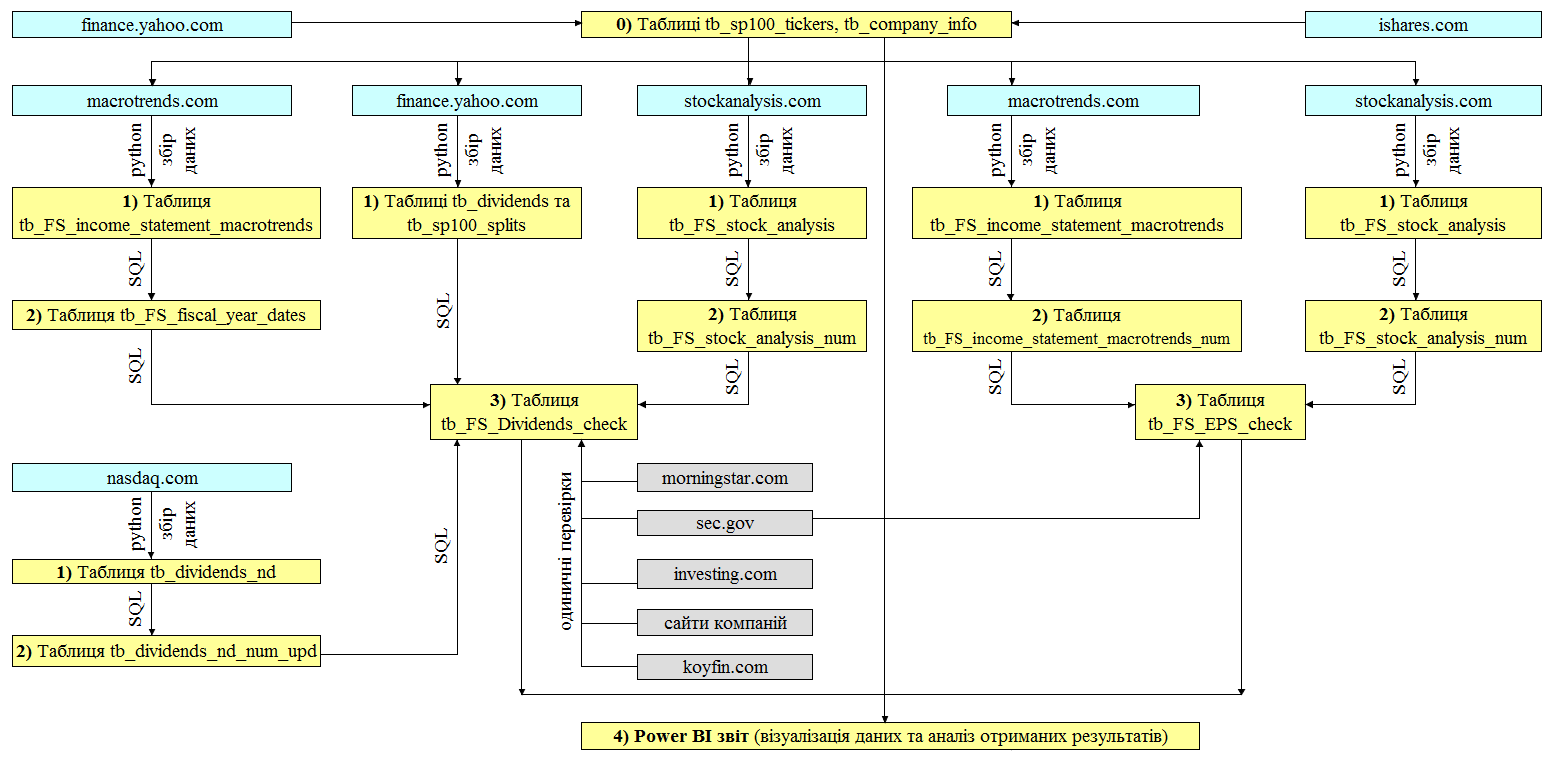
\includegraphics[scale=0.35]{Data Flow full.png}
\end{center}
\end{frame}

\section{Ідентифікація виду дивідендної політики компаній, що входять до індексу Standard \& Poor's 100}
\begin{frame}
\frametitle{Ідентифікація видів дивідендної політики компаній, що входять до індексу Standard \& Poor's 100 (Power BI звіт на прикладі AAPL)}
\begin{center}
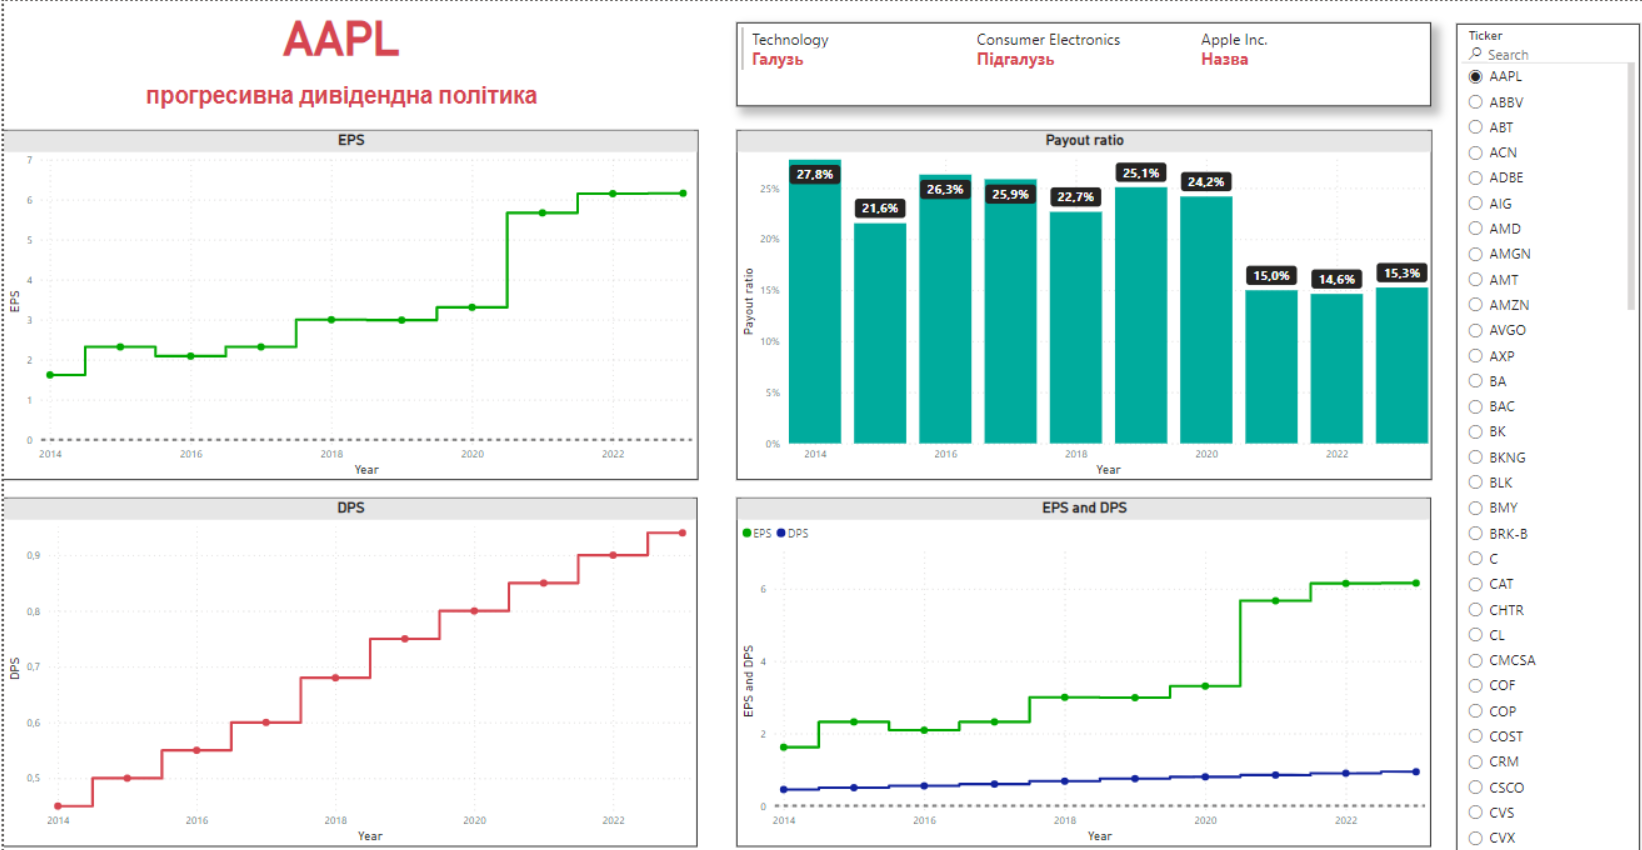
\includegraphics[scale=0.30]{AAPL example.png}
\end{center}
\end{frame}

\begin{frame}
\frametitle{Види дивідендної політики}
\begin{center}
\begin{itemize}
\item  \alert {Результати:} найбільш часто зустрічається прогресивна дивідендна політика (68 випадків), потім нульового дивіденду (15 випадків), найменш популярними є політика фіксованого дивіденду (4 випадки) та регресивна (2 випадки)*
\end{itemize}
\tinyskip
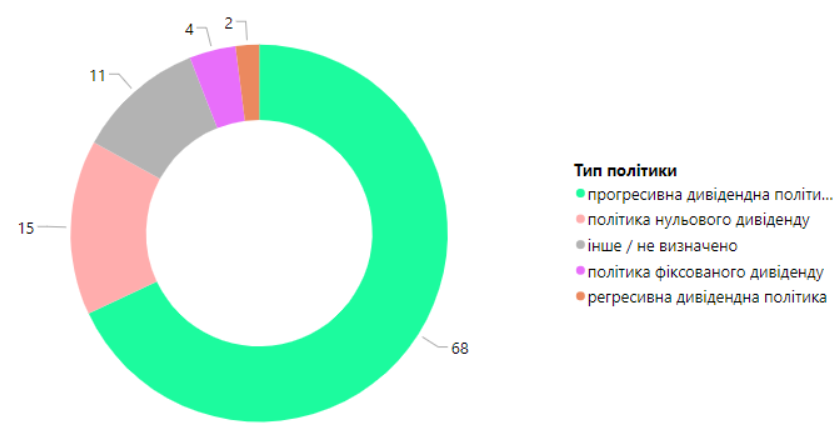
\includegraphics[scale=0.40]{Dividend policy Types.png}
\tinyskip
\end{center}
\scriptsize \textcolor{gray}{*для 11 випадків не вдалося визначити вид дивідендної політики, для жодної з компаній не була притаманна політика стабільного відсотка дивідендних виплат, фіксованого дивіденду з преміальними виплатами, 100\% дивіденду.} 
\end{frame}

\begin{frame}
\frametitle{Зміни в дивідендній політиці протягом досліджуваного періоду}
\begin{center}
\begin{itemize}
\item  \alert {Результати:} для 78 компаній не виявлено використання різних видів дивідендної політики протягом досліджуваного періоду, натомість 22 компанії змінювали дивідендну політику за 2014-2023 роки принаймні одного разу.
\end{itemize} 
\bigskip
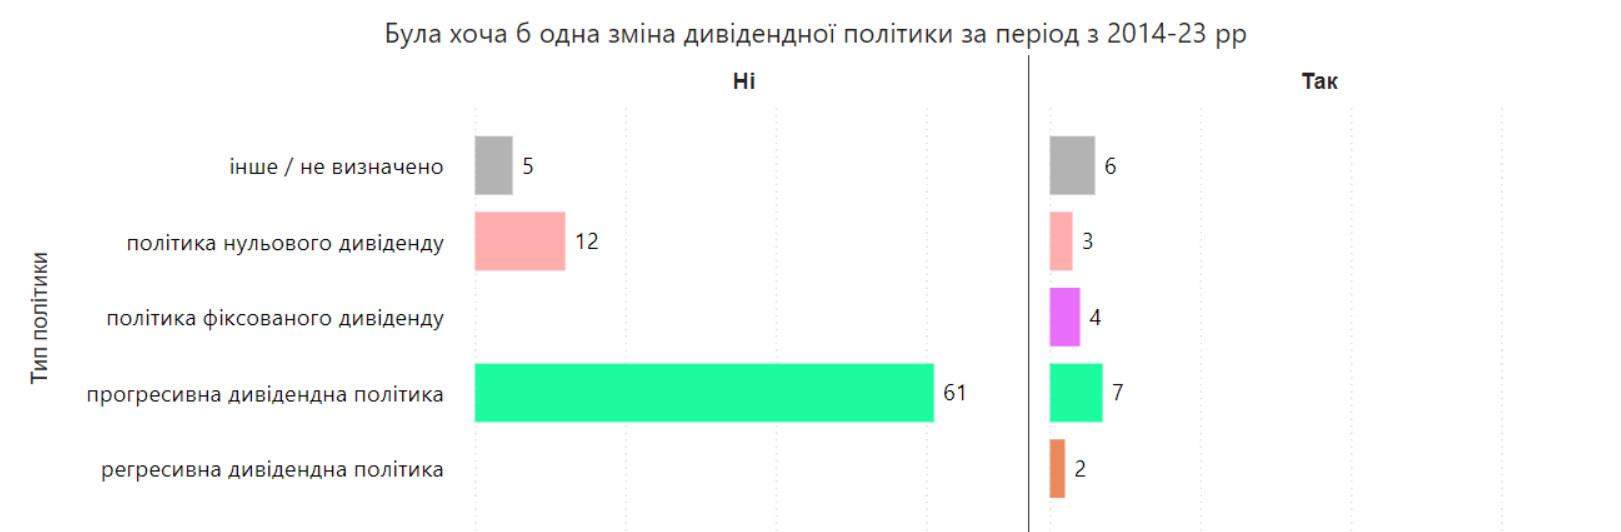
\includegraphics[scale=0.35]{Dividend policy Changes.png}
\end{center}
\end{frame}

\begin{frame}
\frametitle{Випадки, коли DPS >= EPS }
\begin{center}
\begin{itemize}
\item  \alert {Результати:} для 49 компаній за період 2014-2024 років був хоча б один рік, в якому значення DPS перевищує EPS (тобто компанія або спрямовує на виплату дивідендів більше коштів, ніж отримала чистого прибутку, або спрямовує весь чистий прибуток на виплату дивідендів).
\end{itemize}
\bigskip
\includegraphics[scale=0.35]{EPS and DPS comparison.png}
\end{center}
\end{frame}

\begin{frame}
\frametitle{Прогресивна дивідендна політика з преміальними виплатами}
\begin{multicols}{2}
\begin{itemize}
\item На основі аналізу показників COST (Costo Wholesale Corporation) пропонуємо розглянути можливість визначення нового виду дивідендної політики \alert {«прогресивна дивідендна політика з преміальними виплатами»},
\bigskip
\item Він характеризується наявністю чітко вираженого тренду на зростання дивідендів по аналогії з прогресивною дивідендною політикою, але відрізняється наявністю преміальних виплат в особливо успішні роки.
\end{itemize}
\columnbreak
\hspace{5mm}
\includegraphics[scale=0.37]{COST - short.png}
\end{multicols}
\end{frame}

\section{Висновки}

\begin{frame}
\frametitle{Висновки}
\begin{itemize}
\item Для компаній, що
входять до індексу S\&P 100, було зібрано дані за останні 10
років для визначення видів дивідендної політики, процес збору та обробки максимально автоматизовано (python, SQL, Power BI).
\smallskip
\item На основі зібраних даних з використанням критеріїв для визначення основних видів дивідендної політики було \alert {\textbf{визначено види дивідендної політики для кожної з компаній та проаналізовано додаткові характеристики дивідендної політики}}, зокрема зміну дивідендної політики компаніями протягом розглянутого періоду.
\smallskip
\item \alert {\textbf{Запропоновано}} новий вид дивідендної політики \alert {«прогресивна дивідендна політика з преміальними виплатами»} на основі аналізу показників компанії Costo Wholesale Corporation. 
\smallskip
\definecolor{cadmiumgreen}{rgb}{0.0, 0.42, 0.24}
\item \textcolor{blue} {У подальшому доцільно було б розглянути} інші аспекти дивідендної політики, окрім дивідендів в грошовій формі; можливість визначення нового виду дивідендної політики «прогресивна політика з преміальними виплатами»; аналогічні дослідження для більших наборів даних та для інших країн.
\bigskip
\end{itemize}
\end{frame}

\section{Q\&A}

\begin{frame}
\frametitle{Q\&A}
\begin{center}
\bigskip
\textcolor{blue}{\huge Дякую за увагу!} \\
\end{center}
\begin{multicols}{2}

\vbox{\vspace{0.1cm}}
У репозиторії github, \textcolor{blue}{перейти до якого можна відсканувавши QR-код праворуч}, розміщено:
\begin{itemize}
\item скрипти програм для збору і обробки даних, створення таблиць та представлень, розрахунків (.ipynb, .sql, .py)
\item файл Power BI (.pbix)
\item повний бекап бази даних (.bak) 
\end{itemize}
\columnbreak
\hspace{5mm}

\includegraphics[scale=0.35]{QR code.png}
\end{multicols}
\end{frame}

\begin{frame}
\frametitle {Q\&A - Формування дивідендної політики корпорації (на прикладі компаній, що входять до індексу Standard \& Poor's 100 }
\setbeamertemplate{section in toc}[circle]
%\setbeamercolor{section in toc}{fg=UniBlue}
%\setbeamercolor*{section in toc}{fg=UniBlue}
\tableofcontents
\end{frame}

\end{document}